\documentclass[12pt]{article}
\usepackage{esqu1}
\pagestyle{fancy}

\lhead{Brandon Lin}
\chead{Differential Equations}
\rhead{Spring 2016}

\begin{document}
\title{Differential Equations}
\author{Brandon Lin\\Stuyvesant High School\\Spring 2016\\Teacher: Mr. Stern}
\maketitle
\newpage
\section*{Introduction}

\section{2/3/16}
\textbf{Aim}: Background on $\mathbb{R}$; Basic Existence Question of ODE's
\subsection{Romeo and Juliet}
\[
\begin{cases}
R' = aR + bJ \\
J' = cR + dJ 
\end{cases}
\]

These equations model the rate of change of Romeo's and Juliet's feelings. We call this a \textbf{linear system of two coupled differential equations of first order in two unknowns}. 
\begin{itemize}
\item What makes it linear is that the functions and variables appear in a linear fashion. 
\item What makes it coupled is that both equations have both $R$ and $J$ in them.
\item An \textbf{uncoupled system} would look like:
\[
\begin{cases}
R' = aR \\
J' = bJ
\end{cases}
\] 
\item First-order refers to the fact that all the derivatives are the first derivatives.
\end{itemize}
``Identically cautious lovers'':
\[
\begin{aligned} 
R' = aR + bJ &\quad a<0, b>0 \\
J' = bR + aJ &\quad |a| > |b|
\end{aligned}
\]

We may have initial conditions, $R(0)$ and $J(0)$, and plot them on a \textbf{phase plane} with $R$ against $J$. In this case, no matter where the starting point is, the trajectory will go towards a \textbf{stable node}.
\begin{figure}[h!]
\centering
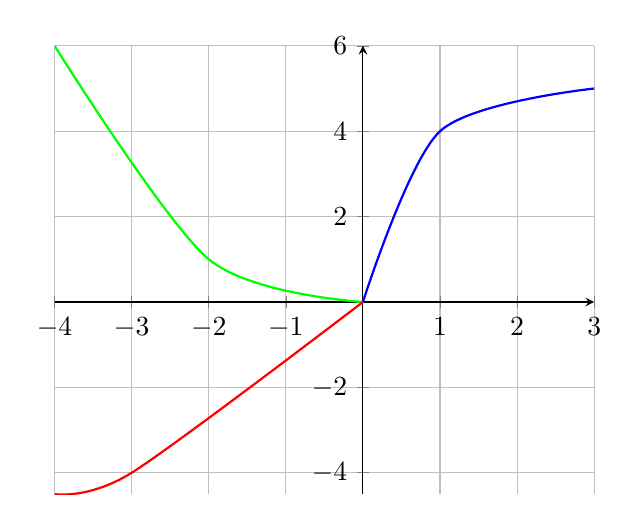
\begin{tikzpicture}
\begin{axis}[grid=major,axis x line=middle,
             axis y line=middle,
             after end axis/.code={
  }]

\addplot[color = green, smooth, thick] coordinates
    {(-4,6) (-2,1) (0,0)};
\addplot[color = blue, smooth, thick] coordinates
    {(3,5) (1,4) (0,0)};
\addplot[color = red, smooth, thick] coordinates
    {(-4,-4.5) (-3,-4) (0,0)};
\end{axis}
\end{tikzpicture}
\end{figure}

In the case of $|a| < |b|$, points will move asymptotically towards $R = -J$ and $R = J$. \\
In the case of $|a| = |b|$, points will cycle around the origin infinitely.
\newpage

\subsection{Supremum and Infimum of a Set $\mathcal{A} \subseteq \mathbb{R}$}
\begin{itemize}
\item If $\mathcal{A} \in (-\infty, b{]}$ for some $b \in \mathbb{R}$, we say $\mathcal{A}$ is bounded above, and that $b$ is an \textbf{upper bound} for $A$. 
\end{itemize}

\begin{theorem}[Supremum Theorem]
If $\mathcal{A} \in \mathbb{R}$, $A \neq \emptyset$, and $A \subseteq (-\infty, b{]}$ for some $b \in \mathbb{R}$, then there exists $a \in \mathbb{R}$ such that $\mathcal{A} \subseteq (-\infty, a {]}$ but if $x < a$, then $\mathcal{A} \not \subseteq (-\infty, x {]}$. \\
We write $a = \sup{\mathcal{A}}$, call it the \textbf{supremum} of $\mathcal{A}$.
\end{theorem}

Why is this necessary? Consider the set $\mathcal{A} = \{-\frac{1}{n} | n \in \mathbb{N} \}$. It does not have a maximum persay, but it has a supremum $\sup{\mathcal{A}} = 0$. \\ \\
Consider this example: What is $\sup{(-\mathbb{N})}$? It is -1, which also happens to be the maximum of the set.

\begin{theorem}
If max $A$ exists as a real number, then $\sup{A} = \max{A}$.
\end{theorem}

But to answer all these questions, we need to figure out: what exactly are the real numbers? 

\subsection{What is $\mathbb{R}$?}
Let $x = (s,N,d_1,d_2,d_3,\dots,d_k,\dots)$, where:
\begin{itemize}
\item $s \in \{+1,-1\}$
\item $N \in \mathbb{Z}$
\item $d_k \in \mathbb{D} = \{0,1,2,3,4,5,6,7,8,9\}$
\item $\neg (\exists k : d_{k+1} = d_{k+2} = \dots = 0)$
\end{itemize}

In this case, ``2.49'' is shorthand for $(+1,2,4,8,9,9,9,\dots)$
\end{document}
